\documentclass{article}
\usepackage[a4paper]{geometry}
\usepackage[skip=10pt]{parskip}
\usepackage{graphicx}
\usepackage{hyperref}
\usepackage[section]{placeins}
\usepackage[official]{eurosym}
\usepackage{textgreek}
\usepackage{tcolorbox}
\usepackage{listings}
\usepackage{textcomp}
\usepackage{multirow}
\usepackage{tikz}

\setlength\parindent{0pt}

\newenvironment{note}{\begin{tcolorbox}[colback=blue!5!white,colframe=blue!75!black,title=\textbf{Note}]}{\end{tcolorbox}}
\newenvironment{caution}{\begin{tcolorbox}[colback=red!5!white,colframe=red!75!black,title=\textbf{Caution}]}{\end{tcolorbox}}
\newcommand{\evaboard}{\href{https://github.com/7vgn/EvaBoard/}{evaluation board}}
\newcommand{\datasheet}{\href{https://ww1.microchip.com/downloads/aemDocuments/documents/MPD/ProductDocuments/DataSheets/23A102423LC1024-1-Mbit-SPI-Serial-SRAM-with-SDI-SQI-Interface-20005142.pdf}{datasheet}}
\newcommand{\CS}{$\overline{\mbox{CS}}$}
\renewcommand{\SS}{$\overline{\mbox{SS}}$}
\newcommand{\file}[1]{\texttt{#1}}

\lstset
{
	basicstyle=\footnotesize\ttfamily,
	breaklines=true,
	keywordstyle=\bfseries\color{green!40!black},
	commentstyle=\itshape\color{purple!40!black},
	identifierstyle=\color{blue},
	stringstyle=\color{orange},
	tabsize=4
}

\begin{document}
\hypersetup{pageanchor=false}
\begin{titlepage}
\thispagestyle{empty}
\centering
\textsf{\Huge Guide Book}\\[1cm]
\textsf{\Large For the SRAM Add-On Board}\\[3cm]
\includegraphics[width=\textwidth]{Pictures/SRAMBoard3DRender.png}
\end{titlepage}
\hypersetup{pageanchor=true}

\tableofcontents
\section{Introduction}
This is an add-on for the ATmega644(A) \evaboard. It is inspired by (and compatible with) the \href{https://www.embedded.rwth-aachen.de/doku.php?id=lehre:atmegaevaboard}{add-on board} used in the lab course "Praktikum Systemprogrammierung" in the computer science curriculum at RWTH Aachen. 

The university encourages students and educators to build the boards themselves. However, the resources it provides are not always the most comprehensive. 

This project provides a complete remake of the original board with a focus on hand-solderable components. It also includes a ton of documentation, especially for students who have not worked with electronics before. 

\begin{note}
Before reading this, you should familiarize yourself with the \evaboard. Many things written there apply here as well and this document can only be considered complete in conjunction with the \href{https://github.com/7vgn/EvaBoard/Guide/EvaBoardGuide.pdf}{evaluation board's Guide Book}.
\end{note}

\subsection{Getting to Know the Add-On Board}\label{sec:boardOverview}
This add-on board features the \href{https://www.microchip.com/en-us/product/23lc1024}{23LC1024 128kByte Static RAM} by Microchip. See Figure \ref{fig:schematic} for the \href{../KiCAD/Schematic.pdf}{schematic}. 
\begin{figure}[htb]
\centering
\includegraphics[width=0.85\textwidth]{Pictures/Schematic.png}
\caption{Schematic of the Board}
\label{fig:schematic}
\end{figure}

The 23LC1024 has an SPI interface (among others). When plugged onto Port B (J12) of the evaluation board, the pins match exactly the SPI pins of the ATmega. In addition to that, the add-on board needs power via J3 which can be obtained from the evaluation board's J3 or J4. LED1 signals activity on the SCK line. 

Table \ref{tab:connections} shows the connections between the ATmega and the 23LC1024 when the add-on board is plugged into the Port B connector of the evaluation board (facing towards the side with the LEDs). Port B4 happens to be the $\overline{\mbox{SS}}$ pin, but this is a coincidence -- this pin is not controlled by the ATmega's SPI module while in master mode. 
\begin{table}
\centering
\begin{tabular}{l|l|l|l|l}
\multicolumn{2}{l|}{\textbf{ATmega644}}&\multicolumn{2}{|l|}{\textbf{23LC1024}}&\multirow{2}{*}{\textbf{Remarks}}\cr\cline{1-4}
\textbf{Pin Name}&\textbf{Function}&\textbf{Pin Number}&\textbf{Pin Name}\cr\hline
Port B0&GPIO&\multicolumn{2}{|c|}{--}&\cr\hline
Port B1&GPIO&\multicolumn{2}{|c|}{--}&\cr\hline
Port B2&GPIO&7&$\overline{\mbox{HOLD}}$/SIO3&Only if JP4 is bridged\cr\hline
Port B3&GPIO&3&SIO2&Only if JP3 remains bridged\cr\hline
Port B4&GPIO&1&\CS&\cr\hline
Port B5&MOSI&5&SI/SIO0&\cr\hline
Port B6&MISO&2&MISO/SIO1&\cr\hline
Port B7&SCK&6&SCK&\cr\hline
\end{tabular}
\caption{Connections between the Add-On Board and the Evaluation Board}
\label{tab:connections}
\end{table}

All pins of Port B are passed through to J2. This way, unused pins and pins that can be shared remain usable. 
Port B0 and B1 are not used at all. Port B2 is used only if the solder jumper JP4 is bridged. Port B3 is only used while the the solder jumper JP3 remains bridged\footnote{JP4 is open and JP3 is closed by default. This is because the orginal board comes in this configuration.}. The SPI pins (Port B5..B7) can be shared with other SPI devices so long as separate pins are used for their \CS. 
\FloatBarrier

\subsection{Changes from the Original Board}\label{sec:differences}
\begin{itemize}
\item The main difference is that this board supports both through-hole (THT) and surface mounted (SMD) components. Both kinds are listed in the \href{../BOM/BOM.pdf}{BOM}. You can mix THT and SMD components. See Figure \ref{fig:thtSmd} for a comparison of the different components. \\
The components had to be moved around quite a bit but the connectors J1 and J2 kept their positions. The board is still fully compatible with the original. 
\item The pass-through header J2 was added so that unused or sharable pins of Port B are available for other applications. In particular, you can add multiple devices on the SPI bus of the ATmega. 
\item The pull-up resistor R4 has been added to the \CS{} line. This prevents the 23LC1024 from being accidentally selected while the ATmega is programmed (and leaves Pin B4 floating). 
\item The solder jumper JP3 was added to disconnect Port B3 from SIO2. This line is only required in SQI mode which the ATmega does not support anyway. You can cut it, thus gaining an additional free microcontroller pin. 
\end{itemize}

\begin{figure}[htb]
\centering
\includegraphics[width=0.85\textwidth]{Pictures/THTSMD.jpg}
\caption{Board with THT components (left) vs. SMD components (right)}
\label{fig:thtSmd}
\end{figure}

\section{Building the Board}
Everything written in the evaluation board's \href{https://github.com/7vgn/EvaBoard/Guide/EvaBoardGuide.pdf}{guide book} applies here as well. This chapter only provides additional information specific to the SRAM add-on board. 

\subsection{Sourcing the 23LC1024}
The 23LC1024 SRAM IC is not easily sourceable in small quantities. Neither Reichelt nor Conrad have it available, and even on marketplaces like eBay or Aliexpress it can be hard to find. You can of course get it from big distributors like Mouser but that comes with disproportionate shipping costs.

Here are some options to look out for:
\begin{itemize}
\item The SMD variant (sometimes named “23LCBT”) seems to have slightly better availability. This PCB supports both DIP and SO-8 (SOIC) packages, but the latter is harder to solder for beginners. 
\item Check for both the normal (-I) and the extended temperature range (-E) variant. While in theory -E should be more expensive, availablity and prices fluctuate.
\item If you don’t need the full 1024 kbit, you can use the 512 kbit version which is pin compatible. The 23LC512 is even available from Reichelt (as SOIC only).
Keep in mind however that you will have to make a slight change to your firmware since the 23LC512 uses 2 rather than 3 address bytes.
\end{itemize}

\begin{caution}
Do not buy the 23\emph{A}1024. It is not 5V-tolerant. 
\end{caution}

\begin{note}
There is an even smaller SMD variant (TSSOP) which the PCB \emph{cannot} accommodate. You might be able to use an SSOP-to-DIP adapter (``breakout board''). However, SSOP is \emph{very hard} to solder by hand -- there is less than half a millimetre of space between adjacent legs. 
\end{note}

\subsection{Soldering SMD Components}
\begin{note}
If you are using through-hole (THT) components, this section is not relevant to you. 
\end{note}

SMD components are somewhat harder to solder due to their size. This board uses the largest SMD components available, but they are still much smaller than their THT counterparts. 

In addition to the standard tools, you need some tweezers (ideally cross-locking) and -- depending on how good your eyesight is -- a magnifying glass. Using flux\footnote{Flux is quite expensive, but you can make your own: Take an empty nail polish remover bottle and fill it with some rosin (colophony) flakes. Rosin is pretty cheap and if you happen to know a violin player, they might give you the tiny amount necessary for free. Add some isopropyl alcohol and let it sit until the rosin dissolves.} makes things much easier. 

Make sure the PCB is clean; use isopropyl alcohol if necessary. It is important that the PCB's metal pads and the solder mask in between are in good condition. Do not solder for more than a few seconds at a time, otherwise you might destroy them. If you have flux, apply some to all the pads of a component before soldering. 

Start by heating one of the pads of the PCB, then add a tiny bit of solder onto it. Grab the component with tweezers and move it in the correct position. Make sure the orientation is correct. Then heat the prepared pad with your soldering iron, while still firmly holding the component in place. Remove the iron and let it cool for a few seconds. The component is now attached on one side (or with one leg). 

It the placement isn't quite right, grab the component with tweezers, re-heat the solder joint and move or rotate slightly. The solder joint doesn't have to be perfect, it just needs to hold the component in place. Once the component is correctly positioned, solder the remaining sides or legs. After that you can re-do the first solder joint if necessary. 

Use only very small amounts of solder. The components should lie flat on the PCB, not swim on top of a big drop of solder. If necessary, remove solder with a soldering pump or wick. 

If the solder bridges neighbouring pins, use wick to remove it. Adding some more flux can also help. 
Finally, clean the PCB with isopropyl alcohol to remove flux residue. 

With SMD components it is even more important to check the connections using a multimeter in continuity testing mode. At the very least verify that the pins of the IC are connected to the corresponding pins of J1 and J3 and that there is no short between neighbouring pins. 

\section{Testing}
The test programs can be found in the \href{../Tests/}{\file{Tests/} subdirectory} of this repository. They all come with makefiles for AVR-GCC and AVRDUDE. Alternatively, you can create a project in your IDE of choice and import the source files there. Be sure to define the \lstinline[language=C]{F_CPU} constant if your IDE doesn't do that automatically.

\subsection{Bit-Banging}\label{sec:bitBang}
The code for this test can be found in \href{../Tests/BitBang/}{\file{Tests/BitBang/}}. 

This test uses a technique called \href{https://en.wikipedia.org/wiki/Bit_banging}{``bit-banging''} to communicate with the SRAM. This means, rather than using the ATmega's SPI peripheral, it generates the required bit sequence on the pins in software. This approach is much slower but it allows for a free choice of the pins: You can attach the add-on board to any port, so long as you change the configuration in \texttt{main.c} accordingly. 

The program uses a pseudo random number generator to choose a 17-bit address and two bytes of data. It then writes the data to the SRAM at that address and tries to read it back again. This is repeated forever or until a discrepancy is found. 

\paragraph{Preparation}
Plug the SRAM board onto Port B (J12) facing towards the side with the LEDs and provide it with power from connector J3 or J4 of the evaluation board. Connect the LCD (J15) to Port A (J11), i.e.\ connect R/W to Port A6, EN to Port A5, RS to Port A4, DB7 to Port A3, DB6 to Port A2, DB5 to Port A1, and DB4 to Port A0. See Figure \ref{fig:bitBang}. 

\begin{figure}[htb]
\centering
\includegraphics[width=0.85\textwidth]{Pictures/BitBang.jpg}
\caption{Setup for the Bit-Banging Test}
\label{fig:bitBang}
\end{figure}

\paragraph{Expected Result}
The LCD should output the currently used address and the data it writes and reads. It should never show ``E'' at the end of the second row. 

\paragraph{Troubleshooting}
Make sure the evaluation board, including the LCD, is working reliably. Re-check all connections. Is the add-on board powered with the correct polarity? 

If all connections are correct and it still doesn't work, then there is either a bad solder joint or the SRAM IC is defective. The LED should flash whenever the SCK line is high, i.e.\ when there's activity on the SPI bus. If it doesn't, there might be a problem with the SCK line. Reading a value of 0xffff indicates that the SRAM is not sending data (the pull-up on Port B6 causes the controller to read ones). This could be because of a problem on the MISO line (but also on the MOSI line, since it is hard to tell whether the SRAM even receives any commands). 

\subsection{Manually Communicating over SPI}
This is not so much a test as it is an opportunity to learn about the SPI protocol. While SPI devices have upper speed limits (see Table 1-2 in the \datasheet), they don't usually have lower limits, meaning you can communicate with them as slowly as you like. So why not try and do it by hand. 

In theory, we could remove the microcontroller altogether and just wire some buttons to the SRAM board. In practice, it would be incredibly tedious to hold and release buttons without slipping up or miscounting. So we're doing it manually but with the help of the microcontroller. 

\paragraph{Preparation}
Set up the LCD and the add-on board just like in the previous test. Add three wires from Pins C0, C1, and C6 to SW1, SW2, and SW3. Compile and program the code from the \href{../Tests/Manual/}{\file{Tests/Manual/} subdirectory}. 

\begin{figure}[htb]
\centering
\includegraphics[width=0.85\textwidth]{Pictures/Manual.jpg}
\caption{Setup for the Manual Test}
\label{fig:manual}
\end{figure}

\paragraph{Expected Result}
Each press of a button flips the corresponding line from high to low or vice versa. SW1 is for MOSI, SW2 for SCK, and SW3 for \CS. The LCD shows a diagram for each of these lines and MISO. 

Figure \ref{fig:spiManualSequence} shows the RDMR sequence (0x05 0x00, see Section 2.5 of the \datasheet{}), which is a short example you can do manually. It also depicts the expected response on MISO (0x40). Read and write instructions are also possible but as they are at least 40 bits long, they require more patience. 


\begin{figure}[htb]
\centering
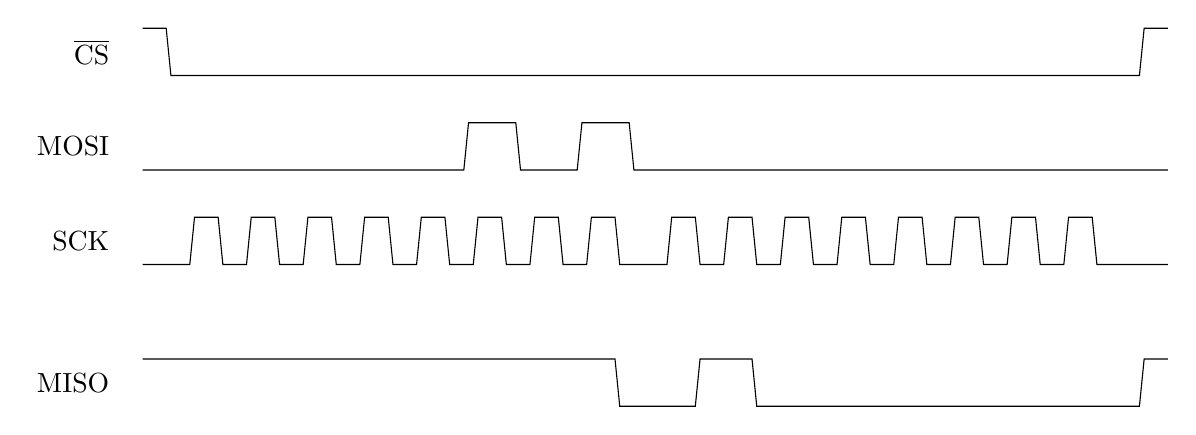
\begin{tikzpicture}[scale=0.6]
\coordinate (CS) at (0,7);
\coordinate (MOSI) at (0,5);
\coordinate (SCK) at (0,3);
\coordinate (MISO) at (0,0);
% CS
\node[anchor=east] at (CS) {\CS};
\draw (CS) ++ (0.5,0.5) -- ++(0.5,0) -- ++(0.1,-1) -- ++(20.5,0) -- ++(0.1,1) -- ++(0.5,0);
% MOSI
\node[anchor=east] at (MOSI) {MOSI};
\draw (MOSI) ++ (0.5,-0.5) -- ++(6.8,0)
-- ++(0.1,1) -- ++(1,0) -- ++(0.1,-1) -- ++(1.2,0)
-- ++(0.1,1) -- ++(1,0) -- ++(0.1,-1) -- ++(11.3,0);
% SCK
\node[anchor=east] at (SCK) {SCK};
\draw (SCK) ++ (0.5,-0.5) -- ++(1,0)
-- ++(0.1,1) -- ++(0.5,0) -- ++(0.1,-1) -- ++(0.5,0)
-- ++(0.1,1) -- ++(0.5,0) -- ++(0.1,-1) -- ++(0.5,0)
-- ++(0.1,1) -- ++(0.5,0) -- ++(0.1,-1) -- ++(0.5,0)
-- ++(0.1,1) -- ++(0.5,0) -- ++(0.1,-1) -- ++(0.5,0)
-- ++(0.1,1) -- ++(0.5,0) -- ++(0.1,-1) -- ++(0.5,0)
-- ++(0.1,1) -- ++(0.5,0) -- ++(0.1,-1) -- ++(0.5,0)
-- ++(0.1,1) -- ++(0.5,0) -- ++(0.1,-1) -- ++(0.5,0)
-- ++(0.1,1) -- ++(0.5,0) -- ++(0.1,-1) -- ++(1,0)
-- ++(0.1,1) -- ++(0.5,0) -- ++(0.1,-1) -- ++(0.5,0)
-- ++(0.1,1) -- ++(0.5,0) -- ++(0.1,-1) -- ++(0.5,0)
-- ++(0.1,1) -- ++(0.5,0) -- ++(0.1,-1) -- ++(0.5,0)
-- ++(0.1,1) -- ++(0.5,0) -- ++(0.1,-1) -- ++(0.5,0)
-- ++(0.1,1) -- ++(0.5,0) -- ++(0.1,-1) -- ++(0.5,0)
-- ++(0.1,1) -- ++(0.5,0) -- ++(0.1,-1) -- ++(0.5,0)
-- ++(0.1,1) -- ++(0.5,0) -- ++(0.1,-1) -- ++(0.5,0)
-- ++(0.1,1) -- ++(0.5,0) -- ++(0.1,-1) -- ++(1.5,0);
% MISO
\node[anchor=east] at (MISO) {MISO};
\draw (MISO) ++ (0.5,0.5) -- ++(10,0)
-- ++(0.1,-1) -- ++(1.6,0) -- ++(0.1,1) -- ++(1.1,0)
-- ++(0.1,-1) -- ++(8.1,0) -- ++(0.1,1) -- ++(0.5,0);
\end{tikzpicture}
\caption{Example Sequence for Manual Test}
\label{fig:spiManualSequence}
\end{figure}

\section{Known Issues}
While the diode is great for preventing damage when the supply voltage is plugged in the wrong way, it causes a violation of the VCC+0.3V maximum input voltage on the 23LC1024's signal lines. So far, we have not observed any problems arising from that. 

\section{Version History}
\begin{description}
\item[v1.0] Initial release
\item[v1.1] Added pull-up resistor R4 for \CS{} and moved JP4 to the back to make space for it. Added JP3 so SIO2 can be disconnected. \\
On v1.0 the pull-up resistor for \CS{} can be soldered to the back, see Figure \ref{fig:csPullupV10}. 
\end{description}

\begin{figure}[htb]
\centering
\includegraphics[width=0.85\textwidth]{Pictures/CSPullupV10.jpg}
\caption{Adding a Pull-up Resistor for \CS{} on v1.0}
\label{fig:csPullupV10}
\end{figure}

\end{document}
